% Sistem yang dijual: Wind Edge Kit di turbin + platform. Turbin dan baterai milik pelanggan.
\documentclass[border=4pt]{standalone}
% Gaya bersama gambar deck Demo Day (dipakai semua gambar/*.tex standalone).
\usepackage{amssymb}
\usepackage{fontspec}
\setmainfont{DejaVu Sans Condensed}
\setsansfont{DejaVu Sans Condensed}
\newfontfamily\judulfont{DejaVu Sans}[BoldFont={DejaVu Sans Bold}, Ligatures=TeX]
\usepackage{tikz,pgfplots}
\pgfplotsset{compat=1.18, every axis/.append style={/pgf/number format/assume math mode=true, /pgf/number format/use comma, /pgf/number format/1000 sep={.}}}
\usetikzlibrary{positioning,arrows.meta,calc,shapes.geometric,fit,backgrounds}
\definecolor{gelap}{HTML}{15242B}
\definecolor{teal}{HTML}{285052}
\definecolor{amber}{HTML}{E8A317}
\definecolor{muda}{HTML}{DCE8E8}
\definecolor{abu}{HTML}{8A9499}
\definecolor{teks}{HTML}{1E2B30}
\definecolor{hijau}{HTML}{2F7D5B}
\definecolor{merah}{HTML}{A33A2A}
\color{teks}
\tikzset{
  ubin/.style={fill=muda, rounded corners=5pt, align=center, inner sep=6pt},
  inti/.style={ubin, fill=gelap, text=white},
  panah/.style={-{Stealth[length=3mm]}, line width=1.3pt, draw=amber},
  panahabu/.style={-{Stealth[length=2.5mm]}, line width=1pt, draw=abu},
  judulubin/.style={font=\judulfont\bfseries},
}
% Dibuat otomatis oleh buat_aset.py dari ml/results/energi_harian.json; jangan diedit manual.
\newcommand{\energiTurbin}{270}
\newcommand{\energiQa}{187}
\newcommand{\energiQb}{377}
\newcommand{\hariEnergi}{140}
\newcommand{\raspiWh}{71}
\newcommand{\chipWh}{4,1}
\newcommand{\raspiPersen}{26}
\newcommand{\chipPersen}{1,5}
\newcommand{\raspiPersenA}{19}
\newcommand{\raspiPersenB}{38}
\newcommand{\raspiPersenNum}{26.3}
\newcommand{\chipPersenNum}{1.5}
\newcommand{\hematKwh}{24}
\newcommand{\kaliHemat}{17}
\newcommand{\jRaspi}{182}
\newcommand{\jChip}{10,4}
\newcommand{\periodeEnergi}{2026-03-31--2026-10-20}

\AtBeginDocument{\hyphenpenalty=10000 \exhyphenpenalty=10000}

\begin{document}
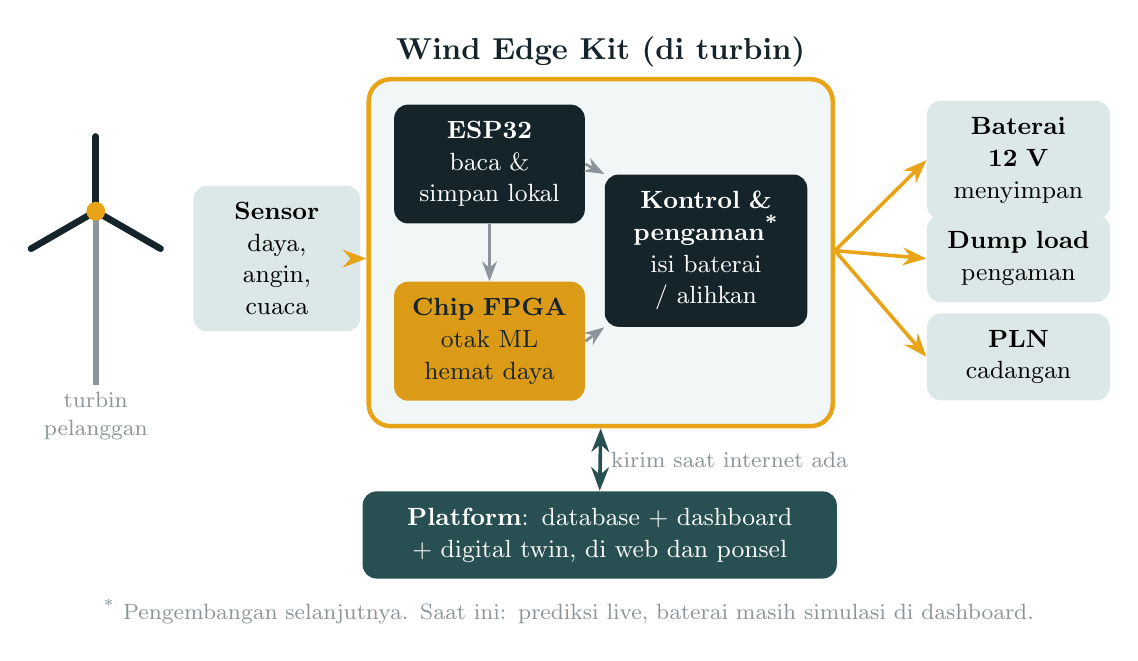
\begin{tikzpicture}[font=\fontsize{9.5}{11.5}\selectfont, node distance=0.45cm]
  % turbin milik pelanggan
  \begin{scope}[shift={(0,0)}]
    \draw[abu, line width=2pt] (0,-1.6) -- (0,0.55);
    \foreach \a in {90,210,330} \draw[gelap, line width=2.4pt, line cap=round] (0,0.6) -- ++(\a:0.95);
    \fill[amber] (0,0.6) circle (0.12);
    \node[align=center, text=abu, font=\fontsize{8.5}{10}\selectfont] at (0,-2.0) {turbin\\pelanggan};
  \end{scope}
  \node[ubin, text width=1.7cm] (sens) at (2.3,0) {\textbf{Sensor}\\daya, angin, cuaca};
  % kotak Wind Edge Kit
  \node[inti, text width=2.0cm] (esp) at (5.0,1.2) {\textbf{ESP32}\\baca \& simpan lokal};
  \node[inti, fill=amber!95!black, text=gelap, text width=2.0cm] (chip) at (5.0,-1.05) {\textbf{Chip FPGA}\\otak ML hemat daya};
  \node[inti, text width=2.15cm] (ctl) at (7.75,0.1) {\textbf{Kontrol \& pengaman\textsuperscript{*}}\\isi baterai / alihkan};
  \begin{scope}[on background layer]
    \node[draw=amber, line width=1.6pt, rounded corners=8pt, fill=muda!40, fit=(esp)(chip)(ctl), inner sep=9pt, label={[font=\judulfont\bfseries\fontsize{10.5}{12}\selectfont, text=gelap]above:Wind Edge Kit (di turbin)}] (kit) {};
  \end{scope}
  \draw[panah] (sens) -- (sens -| kit.west);
  \draw[panahabu] (esp) -- (chip);
  \draw[panahabu] (chip.east) -- (ctl.south west);
  \draw[panahabu] (esp.east) -- (ctl.north west);
  % keluaran energi
  \node[ubin, text width=1.9cm, anchor=west] (baterai) at (10.55,1.25) {\textbf{Baterai 12 V}\\menyimpan};
  \node[ubin, text width=1.9cm, anchor=west] (dump) at (10.55,0.0) {\textbf{Dump load}\\pengaman};
  \node[ubin, text width=1.9cm, anchor=west] (pln) at (10.55,-1.25) {\textbf{PLN}\\cadangan};
  \foreach \t in {baterai,dump,pln} \draw[panah] (kit.east |- ctl) -- (\t.west);
  % platform
  \node[ubin, fill=teal, text=white, text width=5.6cm, anchor=north] (plat) at (6.4,-2.95) {\textbf{Platform}: database + dashboard + digital twin, di web dan ponsel};
  \draw[panah, draw=teal, {Stealth[length=3mm]}-{Stealth[length=3mm]}] (kit.south) -- node[right, font=\fontsize{8.5}{10}\selectfont, text=abu] {kirim saat internet ada} (plat.north);
  \node[anchor=north, text=abu, text width=12.5cm, align=center, font=\fontsize{8.5}{10}\selectfont] at ([yshift=-4pt]current bounding box.south) {\textsuperscript{*} Pengembangan selanjutnya. Saat ini: prediksi live, baterai masih simulasi di dashboard.};
\end{tikzpicture}
\end{document}
